\section{Remoção de elementos em árvores binárias de busca}


\begin{frame}[fragile]{Remoção em árvores binárias de busca}

    \begin{itemize}
	    \item A remoção em árvores binárias { depende da posição do nó} a ser removido

        \item São { três} casos:

        \begin{enumerate}
            \item o nó é uma folha, isto é, não tem filhos

            \item o nó tem um filho

            \item o nó tem dois filhos
        \end{enumerate}

        \item No primeiro caso, basta { remover} a referência do pai e {remover} o nó

        \item No segundo caso, a referência do { pai} é alterada para apontar para neto, e o nó é removido

        \item O terceiro caso não pode ser resolvido em um único passo

        \item Duas possíveis soluções são a remoção por fusão ou a remoção por cópia
    \end{itemize}
\end{frame} 

\begin{frame}[fragile]{Exemplo de remoção de nó sem filhos}

    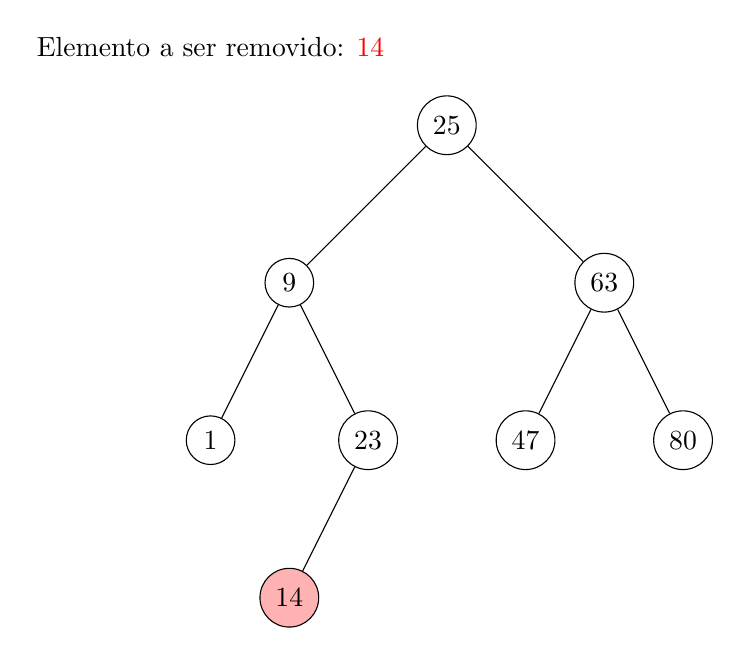
\begin{tikzpicture}

        \begin{scope}{shift={(3,1)}}
            \node (X) at (1, 6) { Elemento a ser removido: \textcolor{red}{14}};

            \node[circle,draw] (D) at (4, 5) { $25$ };
            \node[circle,draw] (C) at (2, 3) { $9$ };
            \node[circle,draw] (E) at (6, 3) { $63$ };
            \node[circle,draw] (F) at (5, 1) { $47$ };
            \node[circle,draw] (A) at (1, 1) { $1$ };
            \node[circle,draw] (B) at (3, 1) { $23$ };
            \node[circle,draw] (G) at (7, 1) { $80$ };
            \node[circle,draw,fill=red!30] (H) at (2, -1) { $14$ };

            \draw (A) -- (C);
            \draw (B) -- (C);
            \draw (C) -- (D);
            \draw (D) -- (E);
            \draw (E) -- (F);
            \draw (E) -- (G);
            \draw (B) -- (H);

        \end{scope}
    \end{tikzpicture}

\end{frame}

\begin{frame}[fragile]{Exemplo de remoção de nó sem filhos}

    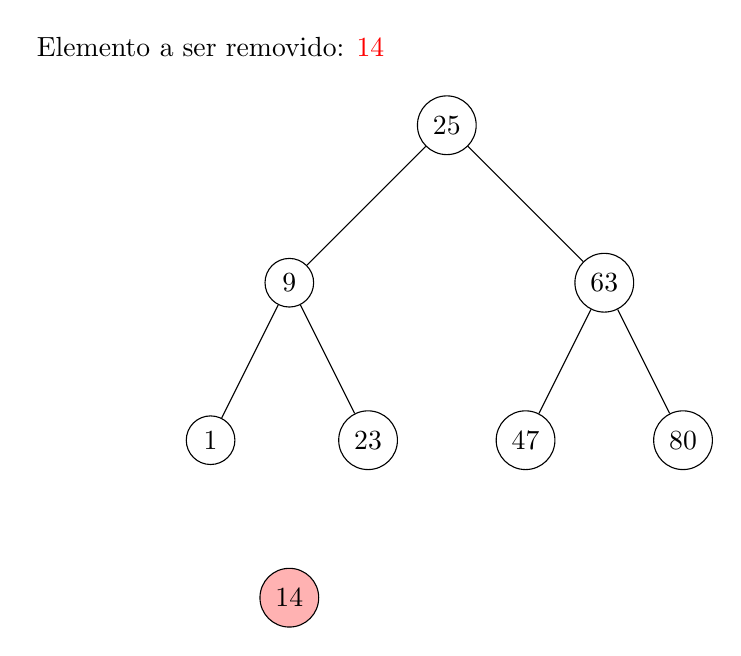
\begin{tikzpicture}

        \begin{scope}{shift={(3,1)}}
            \node (X) at (1, 6) { Elemento a ser removido: \textcolor{red}{14}};

            \node[circle,draw] (D) at (4, 5) { $25$ };
            \node[circle,draw] (C) at (2, 3) { $9$ };
            \node[circle,draw] (E) at (6, 3) { $63$ };
            \node[circle,draw] (F) at (5, 1) { $47$ };
            \node[circle,draw] (A) at (1, 1) { $1$ };
            \node[circle,draw] (B) at (3, 1) { $23$ };
            \node[circle,draw] (G) at (7, 1) { $80$ };
            \node[circle,draw,fill=red!30] (H) at (2, -1) { $14$ };

            \draw (A) -- (C);
            \draw (B) -- (C);
            \draw (C) -- (D);
            \draw (D) -- (E);
            \draw (E) -- (F);
            \draw (E) -- (G);
%            \draw (B) -- (H);

        \end{scope}
    \end{tikzpicture}

\end{frame}

\begin{frame}[fragile]{Exemplo de remoção de nó sem filhos}

    \begin{tikzpicture}

        \begin{scope}{shift={(3,1)}}
            \node (X) at (1, 6) { Elemento a ser removido: \textcolor{black}{13}};

            \node[circle,draw] (D) at (4, 5) { $25$ };
            \node[circle,draw] (C) at (2, 3) { $9$ };
            \node[circle,draw] (E) at (6, 3) { $63$ };
            \node[circle,draw] (F) at (5, 1) { $47$ };
            \node[circle,draw] (A) at (1, 1) { $1$ };
            \node[circle,draw] (B) at (3, 1) { $23$ };
            \node[circle,draw] (G) at (7, 1) { $80$ };
            \node[opacity=0,circle,draw,fill=red!30] (H) at (2, -1) { $14$ };

            \draw (A) -- (C);
            \draw (B) -- (C);
            \draw (C) -- (D);
            \draw (D) -- (E);
            \draw (E) -- (F);
            \draw (E) -- (G);
%            \draw (B) -- (H);

        \end{scope}
    \end{tikzpicture}

\end{frame}

\begin{frame}[fragile]{Exemplo de remoção de nó com apenas um filho}

    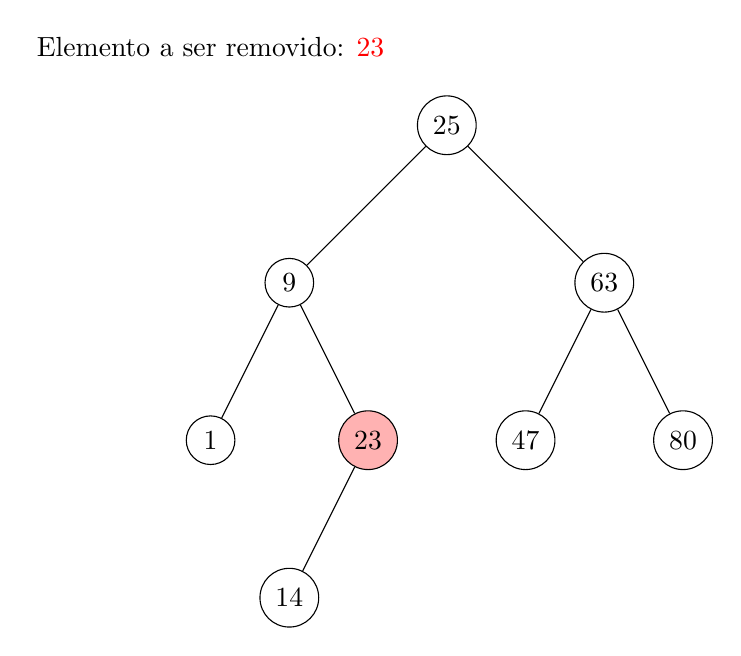
\begin{tikzpicture}

        \begin{scope}{shift={(3,1)}}
            \node (X) at (1, 6) { Elemento a ser removido: \textcolor{red}{23}};

            \node[circle,draw] (D) at (4, 5) { $25$ };
            \node[circle,draw] (C) at (2, 3) { $9$ };
            \node[circle,draw] (E) at (6, 3) { $63$ };
            \node[circle,draw] (F) at (5, 1) { $47$ };
            \node[circle,draw] (A) at (1, 1) { $1$ };
            \node[circle,draw,fill=red!30] (B) at (3, 1) { $23$ };
            \node[circle,draw] (G) at (7, 1) { $80$ };
            \node[circle,draw] (H) at (2, -1) { $14$ };

            \draw (A) -- (C);
            \draw (B) -- (C);
            \draw (C) -- (D);
            \draw (D) -- (E);
            \draw (E) -- (F);
            \draw (E) -- (G);
            \draw (B) -- (H);

        \end{scope}
    \end{tikzpicture}

\end{frame}

\begin{frame}[fragile]{Exemplo de remoção de nó com apenas um filho}

    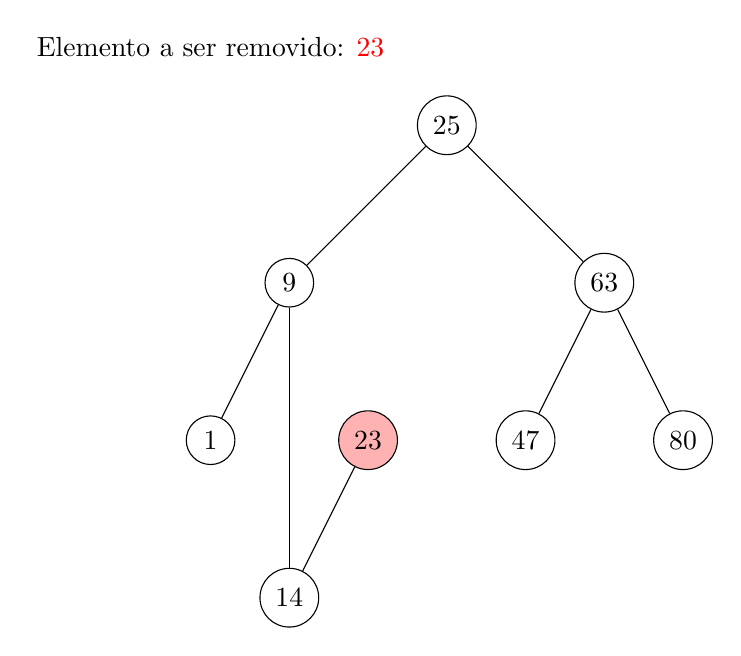
\begin{tikzpicture}

        \begin{scope}{shift={(3,1)}}
            \node (X) at (1, 6) { Elemento a ser removido: \textcolor{red}{23}};

            \node[circle,draw] (D) at (4, 5) { $25$ };
            \node[circle,draw] (C) at (2, 3) { $9$ };
            \node[circle,draw] (E) at (6, 3) { $63$ };
            \node[circle,draw] (F) at (5, 1) { $47$ };
            \node[circle,draw] (A) at (1, 1) { $1$ };
            \node[circle,draw,fill=red!30] (B) at (3, 1) { $23$ };
            \node[circle,draw] (G) at (7, 1) { $80$ };
            \node[circle,draw] (H) at (2, -1) { $14$ };

            \draw (A) -- (C);
            \draw (H) -- (C);
            \draw (C) -- (D);
            \draw (D) -- (E);
            \draw (E) -- (F);
            \draw (E) -- (G);
            \draw (B) -- (H);

        \end{scope}
    \end{tikzpicture}

\end{frame}

\begin{frame}[fragile]{Exemplo de remoção de nó com apenas um filho}

    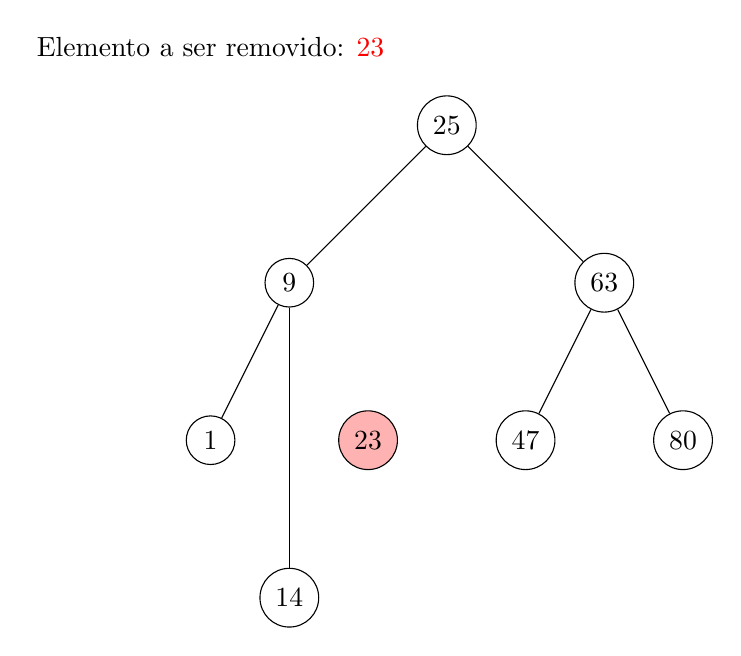
\begin{tikzpicture}

        \begin{scope}{shift={(3,1)}}
            \node (X) at (1, 6) { Elemento a ser removido: \textcolor{red}{23}};

            \node[circle,draw] (D) at (4, 5) { $25$ };
            \node[circle,draw] (C) at (2, 3) { $9$ };
            \node[circle,draw] (E) at (6, 3) { $63$ };
            \node[circle,draw] (F) at (5, 1) { $47$ };
            \node[circle,draw] (A) at (1, 1) { $1$ };
            \node[circle,draw,fill=red!30] (B) at (3, 1) { $23$ };
            \node[circle,draw] (G) at (7, 1) { $80$ };
            \node[circle,draw] (H) at (2, -1) { $14$ };

            \draw (A) -- (C);
            \draw (H) -- (C);
            \draw (C) -- (D);
            \draw (D) -- (E);
            \draw (E) -- (F);
            \draw (E) -- (G);
%            \draw (B) -- (H);

        \end{scope}
    \end{tikzpicture}

\end{frame}

\begin{frame}[fragile]{Exemplo de remoção de nó com apenas um filho}

    \begin{tikzpicture}

        \begin{scope}{shift={(3,1)}}
            \node (X) at (1, 6) { Elemento a ser removido: \textcolor{black}{23}};

            \node[circle,draw] (D) at (4, 5) { $25$ };
            \node[circle,draw] (C) at (2, 3) { $9$ };
            \node[circle,draw] (E) at (6, 3) { $63$ };
            \node[circle,draw] (F) at (5, 1) { $47$ };
            \node[circle,draw] (A) at (1, 1) { $1$ };
            \node[opacity=0,circle,draw,fill=red!30] (B) at (3, 1) { $23$ };
            \node[circle,draw] (G) at (7, 1) { $80$ };
            \node[circle,draw] (H) at (2, -1) { $14$ };

            \draw (A) -- (C);
            \draw (H) -- (C);
            \draw (C) -- (D);
            \draw (D) -- (E);
            \draw (E) -- (F);
            \draw (E) -- (G);
%            \draw (B) -- (H);

        \end{scope}
    \end{tikzpicture}

\end{frame}

\begin{frame}[fragile]\frametitle{Remoção por fusão}

	\begin{itemize}
		\item Esta técnica consiste em gerar uma nova árvore a partir das duas subárvores do nó a 
            ser removido

		\item Numa árvore binária de busca, qualquer elemento da subárvore à direita é maior do 
            que qualquer elemento da subárvore à esquerda

		\item Desta maneira, basta encontrar o nó mais à direita da subárvore à esquerda e 
            transformá-lo no pai da subárvore à direita

        \item São quatro passos para a remoção por fusão:

        \begin{enumerate}
            \item Localize o nó que deve ser removido (com dois filhos) e seu pai

            \item Na subárvore à esquerda, encontre o elemento mais à direita possível: 
                basta mover-se sempre para a direita até que se encontre um nó nulo

            \item Torne a raiz da subárvore à esquerda o novo filho do pai do nó a ser removido 

            \item Faça com que o nó mais à direita da subárvore à esquerda tenha como filho à 
                direita a subárvore à direita do nó a ser removido
        \end{enumerate}

        \item \textit{Corner case}: caso o nó seja a raiz, após a remoção a raiz deve apontar 
            para a raiz da subárvore à esquerda
    \end{itemize}

\end{frame}

\begin{frame}[fragile]{Exemplo de remoção por fusão}

    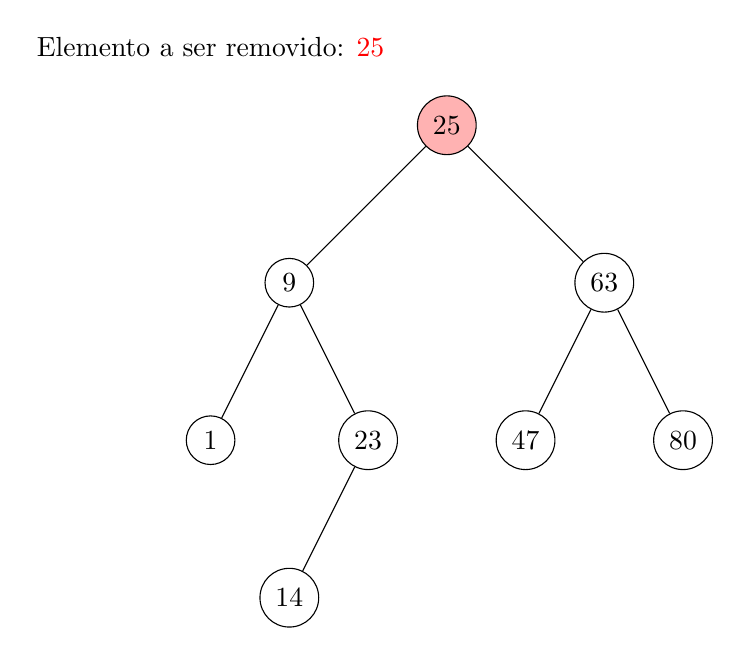
\begin{tikzpicture}

        \begin{scope}{shift={(3,1)}}
            \node (X) at (1, 6) { Elemento a ser removido: \textcolor{red}{25}};

            \node[circle,draw,fill=red!30] (D) at (4, 5) { $25$ };
            \node[circle,draw] (C) at (2, 3) { $9$ };
            \node[circle,draw] (E) at (6, 3) { $63$ };
            \node[circle,draw] (F) at (5, 1) { $47$ };
            \node[circle,draw] (A) at (1, 1) { $1$ };
            \node[circle,draw] (B) at (3, 1) { $23$ };
            \node[circle,draw] (G) at (7, 1) { $80$ };
            \node[circle,draw] (H) at (2, -1) { $14$ };

            \draw (A) -- (C);
            \draw (B) -- (C);
            \draw (C) -- (D);
            \draw (D) -- (E);
            \draw (E) -- (F);
            \draw (E) -- (G);
            \draw (B) -- (H);

        \end{scope}
    \end{tikzpicture}

\end{frame}

\begin{frame}[fragile]{Exemplo de remoção por fusão}

    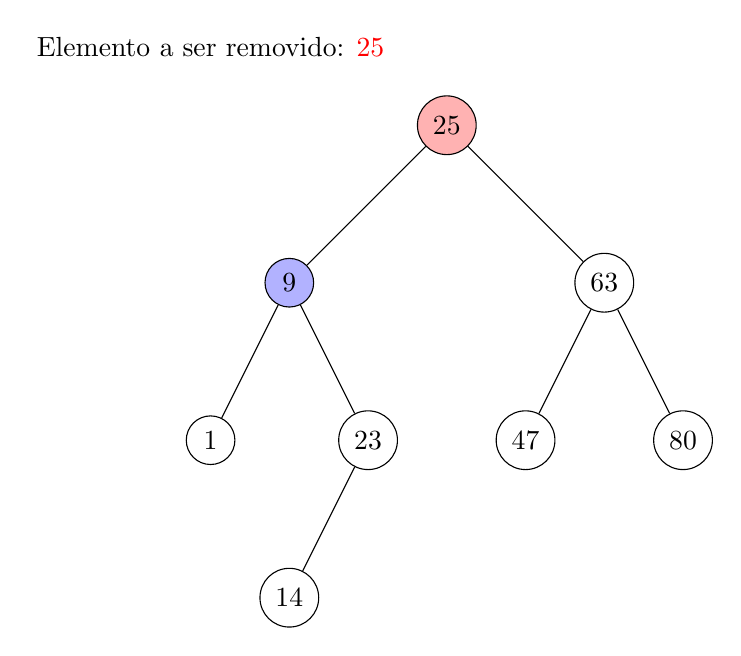
\begin{tikzpicture}

        \begin{scope}{shift={(3,1)}}
            \node (X) at (1, 6) { Elemento a ser removido: \textcolor{red}{25}};

            \node[circle,draw,fill=red!30] (D) at (4, 5) { $25$ };
            \node[circle,draw,fill=blue!30] (C) at (2, 3) { $9$ };
            \node[circle,draw] (E) at (6, 3) { $63$ };
            \node[circle,draw] (F) at (5, 1) { $47$ };
            \node[circle,draw] (A) at (1, 1) { $1$ };
            \node[circle,draw] (B) at (3, 1) { $23$ };
            \node[circle,draw] (G) at (7, 1) { $80$ };
            \node[circle,draw] (H) at (2, -1) { $14$ };

            \draw (A) -- (C);
            \draw (B) -- (C);
            \draw (C) -- (D);
            \draw (D) -- (E);
            \draw (E) -- (F);
            \draw (E) -- (G);
            \draw (B) -- (H);

        \end{scope}
    \end{tikzpicture}

\end{frame}

\begin{frame}[fragile]{Exemplo de remoção por fusão}

    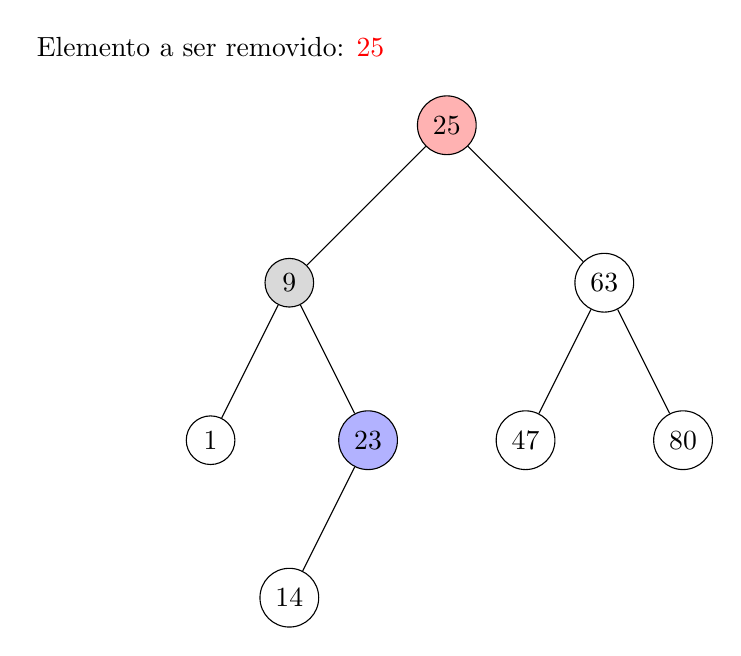
\begin{tikzpicture}

        \begin{scope}{shift={(3,1)}}
            \node (X) at (1, 6) { Elemento a ser removido: \textcolor{red}{25}};

            \node[circle,draw,fill=red!30] (D) at (4, 5) { $25$ };
            \node[circle,draw,fill=gray!30] (C) at (2, 3) { $9$ };
            \node[circle,draw] (E) at (6, 3) { $63$ };
            \node[circle,draw] (F) at (5, 1) { $47$ };
            \node[circle,draw] (A) at (1, 1) { $1$ };
            \node[circle,draw,fill=blue!30] (B) at (3, 1) { $23$ };
            \node[circle,draw] (G) at (7, 1) { $80$ };
            \node[circle,draw] (H) at (2, -1) { $14$ };

            \draw (A) -- (C);
            \draw (B) -- (C);
            \draw (C) -- (D);
            \draw (D) -- (E);
            \draw (E) -- (F);
            \draw (E) -- (G);
            \draw (B) -- (H);

        \end{scope}
    \end{tikzpicture}

\end{frame}

\begin{frame}[fragile]{Exemplo de remoção por fusão}

    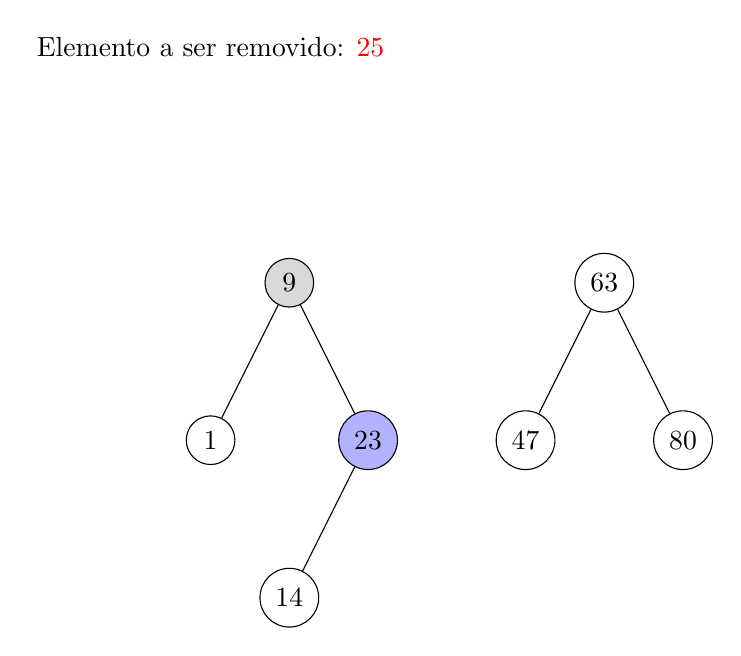
\begin{tikzpicture}

        \begin{scope}{shift={(3,1)}}
            \node (X) at (1, 6) { Elemento a ser removido: \textcolor{red}{25}};

            \node[opacity=0,circle,draw,fill=red!30] (D) at (4, 5) { $25$ };
            \node[circle,draw,fill=gray!30] (C) at (2, 3) { $9$ };
            \node[circle,draw] (E) at (6, 3) { $63$ };
            \node[circle,draw] (F) at (5, 1) { $47$ };
            \node[circle,draw] (A) at (1, 1) { $1$ };
            \node[circle,draw,fill=blue!30] (B) at (3, 1) { $23$ };
            \node[circle,draw] (G) at (7, 1) { $80$ };
            \node[circle,draw] (H) at (2, -1) { $14$ };

            \draw (A) -- (C);
            \draw (B) -- (C);
%            \draw (C) -- (D);
%            \draw (D) -- (E);
            \draw (E) -- (F);
            \draw (E) -- (G);
            \draw (B) -- (H);

        \end{scope}
    \end{tikzpicture}

\end{frame}

\begin{frame}[fragile]{Exemplo de remoção por fusão}

    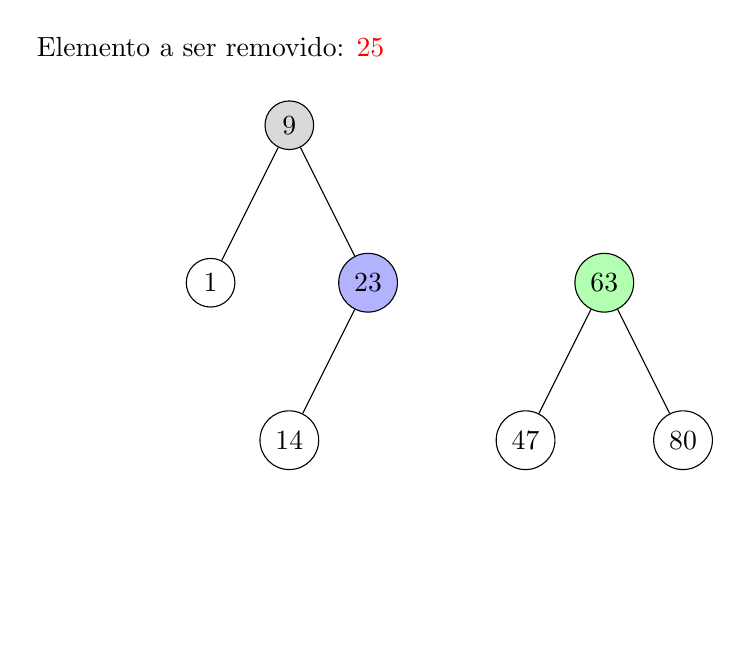
\begin{tikzpicture}

        \begin{scope}{shift={(3,1)}}
            \node (X) at (1, 6) { Elemento a ser removido: \textcolor{red}{25}};

            \node[opacity=0,circle,draw,fill=red!30] (D) at (4, 5) { $25$ };
            \node[circle,draw,fill=gray!30] (C) at (2, 5) { $9$ };
            \node[circle,draw,fill=green!30] (E) at (6, 3) { $63$ };
            \node[circle,draw] (F) at (5, 1) { $47$ };
            \node[circle,draw] (A) at (1, 3) { $1$ };
            \node[circle,draw,fill=blue!30] (B) at (3, 3) { $23$ };
            \node[circle,draw] (G) at (7, 1) { $80$ };
            \node[circle,draw] (H) at (2, 1) { $14$ };
            \node[opacity=0,circle,draw] (I) at (2, -1) { $14$ };

            \draw (A) -- (C);
            \draw (B) -- (C);
%            \draw (C) -- (D);
%            \draw (D) -- (E);
            \draw (E) -- (F);
            \draw (E) -- (G);
            \draw (B) -- (H);

        \end{scope}
    \end{tikzpicture}

\end{frame}

\begin{frame}[fragile]{Exemplo de remoção por fusão}

    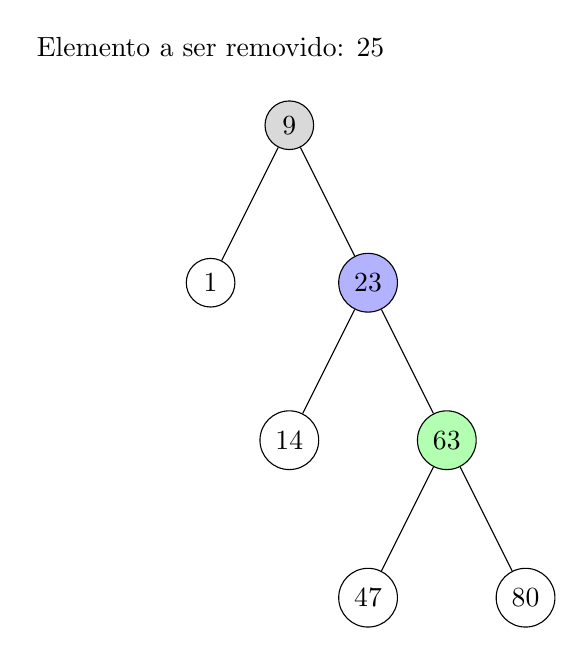
\begin{tikzpicture}

        \begin{scope}{shift={(3,1)}}
            \node (X) at (1, 6) { Elemento a ser removido: \textcolor{black}{25}};

            \node[opacity=0,circle,draw,fill=red!30] (D) at (4, 5) { $25$ };
            \node[circle,draw,fill=gray!30] (C) at (2, 5) { $9$ };
            \node[circle,draw,fill=green!30] (E) at (4, 1) { $63$ };
            \node[circle,draw] (F) at (3, -1) { $47$ };
            \node[circle,draw] (A) at (1, 3) { $1$ };
            \node[circle,draw,fill=blue!30] (B) at (3, 3) { $23$ };
            \node[circle,draw] (G) at (5, -1) { $80$ };
            \node[circle,draw] (H) at (2, 1) { $14$ };
            \node[opacity=0,circle,draw] (I) at (2, -1) { $14$ };

            \draw (A) -- (C);
            \draw (B) -- (C);
            \draw (B) -- (E);
%            \draw (D) -- (E);
            \draw (E) -- (F);
            \draw (E) -- (G);
            \draw (B) -- (H);

        \end{scope}
    \end{tikzpicture}

\end{frame}


\begin{frame}[fragile]{Implementação da remoção por fusão}
    \inputsnippet{cpp}{1}{20}{delete_by_merging.cpp}
\end{frame}

\begin{frame}[fragile]{Implementação da remoção por fusão}
    \inputsnippet{cpp}{21}{37}{delete_by_merging.cpp}
\end{frame}

\begin{frame}[fragile]{Implementação da remoção por fusão}
    \inputsnippet{cpp}{38}{58}{delete_by_merging.cpp}
\end{frame}

\subsection{Remoção por cópia}
\begin{frame}

	\frametitle{Notas sobre a remoção por cópia}

	\begin{itemize}
		\item Algoritmo proposto por { Donald Knuth} e { Thomas Hibbard}.

		\item Ele reduz o caso de um nó ter { dois} filhos para um dos casos anteriores: ou o nó { não tem} 
		filhos ou tem apenas { um}.

		\item Isto é feito { substituíndo} a informação do nó a ser deletado pela informação do nó mais à 
		{ direita} da subárvore { esquerda} e apagando { este nó}.
	\end{itemize}
\end{frame}


%%%%%%%%%%%%%%%%%%%%%%%%%%%%%%%%%%%%%%%%%%%%%%%%%%%%%%%%%%%%%%%%%%%%%%%%%%%%%%%%%%%%%%%%%%%%%%%%%%%%%%%%%%%%%%%%%%%
\begin{frame}

	\frametitle{Remoção por cópia}

	\begin{enumerate}
		\item Localize o nó que deve ser { removido} e que tenha { dois} filhos.

		\item Na subárvore da { esquerda}, encontre o elemento mais a { direita} possível: basta mover sempre 
			a direita até que se encontre um nó { nulo}.

		\item { Substitua} a informação do nó { a ser removido} pela informação do nó localizado no { passo 
		anterior}.

		\item { Remova} o nó localizado no { segundo passo}.
	\end{enumerate}

\end{frame}  

%%%%%%%%%%%%%%%%%%%%%%%%%%%%%%%%%%%%%%%%%%%%%%%%%%%%%%%%%%%%%%%%%%%%%%%%%%%%%%%%%%%%%%%%%%%%%%%%%%%%%%%%%%%%%%%%%%%
%\input{deletebycopying.cpp}
